\documentclass[../Article_Model_Parameters.tex]{subfiles}
\graphicspath{{\subfix{../Figures/}}}
\begin{document}
	
	\label{CH: Results}

    The parameter estimation problem was solved by fitting the process model to the dataset \ref{tab: Yield_data}. Each time-series was fitted to the model separately. As a result of fitting, the following parameters were obtained:

    \begin{itemize}
        \item Partition coefficient $k_m$
        \item Internal Diffusion coefficient $D_i$
        \item Axial Diffusion coefficient $D_e^M$
        \item Standard Deviation $\sigma$
    \end{itemize}

    Moreover, the initial state estimation was performed together with parameter estimation. The concentration of solute is assumed to be constant and uniformly distributed. On the other hand, the solute concentration is assumed to not be uniform and not zero, which is common assumption. During the preparation period, when the operating conditions are achieved, the solute diffuses to the fluid phase in contact with the solid particles. Later, the solute in fluid phase is partially moved (if the pressure increase to the system the pump cause the movement of the fluid, even if the outlet valve is closed) to the region, where there is no solid phase. As a result, the distribution of solute in the fluid phase should be also estimated as it is unknown. Some conclusion can be drown from analysis of the initial part of each yield curve. It can be noticed, that each curve at the beginning has a curvature, which is not linear. In general sens, it can be said that a quadratic function could approximate initial part of each extraction curve. A function which after integration gives a quadratic-like result is a straight line. Based on that observation, the concentration of solute in fluid phase is assumed to be linearly distributed. The concentration of solute is assumed to be zero, at the outlet and reach maximum at beginning of the fixed bed. Such a formulation allows to fully describe the linear distribution of solute in the solid phase if the total mass of solute in the fluid phase is know, as explained in appendix \todo[]{Add chapter}. The total mass of solute in the fluid phase can be obtained from the total mass of solute $m_{total}$ and partition coefficient $\tau$, which is defined as

    {\footnotesize
    \begin{equation*}
        \tau = \cfrac{\text{total mass of solute in the fluid phase}}{\text{total mass of solute in the system}} = \cfrac{m^0_{fluid}}{m_{total}}
    \end{equation*}
    }

    Due to initial state estimation, two additional parameters are fitted

    \begin{itemize}
        \item Total mass of solute $m_{total}$
        \item Partition coefficient $\tau$
    \end{itemize}
	
	Some results of the parameter estimations

	\begin{figure*}
		\centering
		\begin{subfigure}[b]{0.7\textwidth}
			\centering
			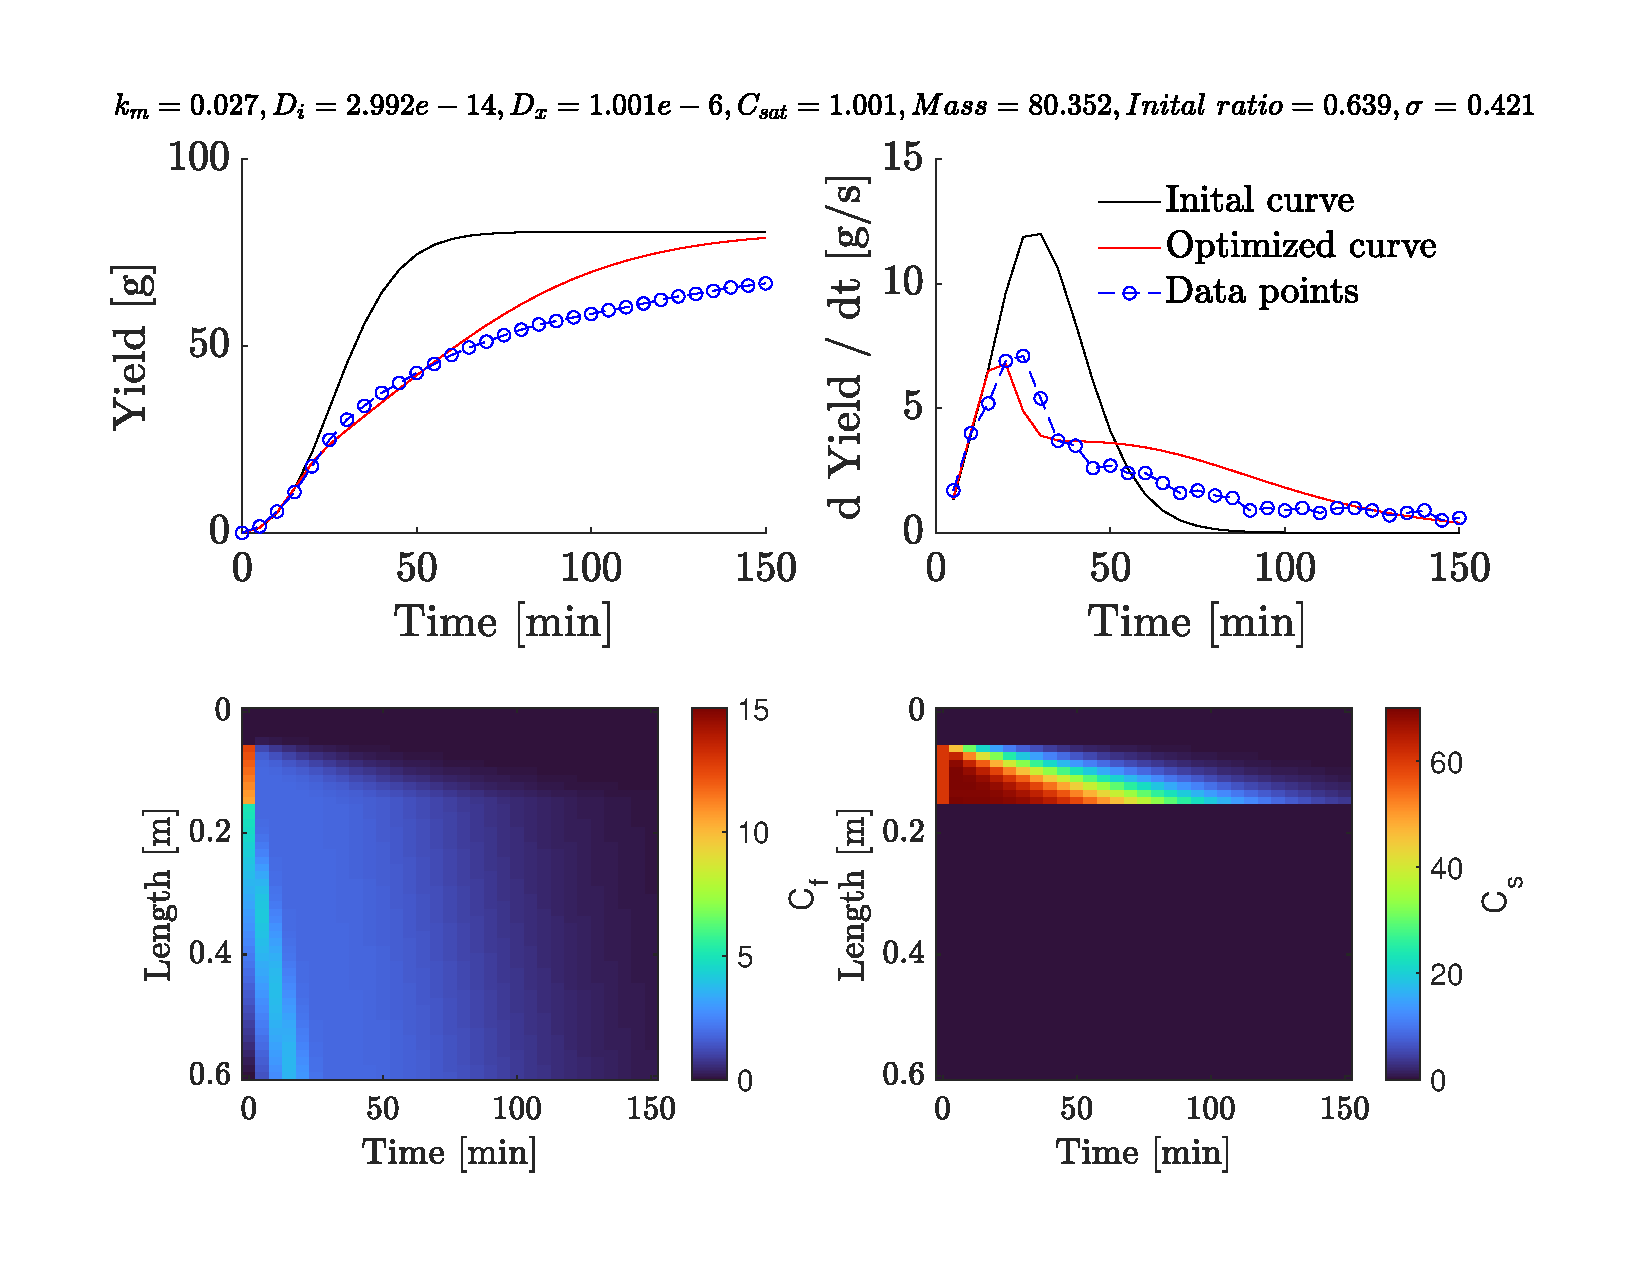
\includegraphics[trim = 3cm 11cm 2.5cm 1cm,clip,width=\textwidth]{/Results_estimation/Fitting_LUKE_T40_P200.pdf}
			\caption{Experiment at $40^\circ C$ and $200$ bar}
		\end{subfigure}
		\hfill
		\begin{subfigure}[b]{0.7\textwidth}
			\centering
			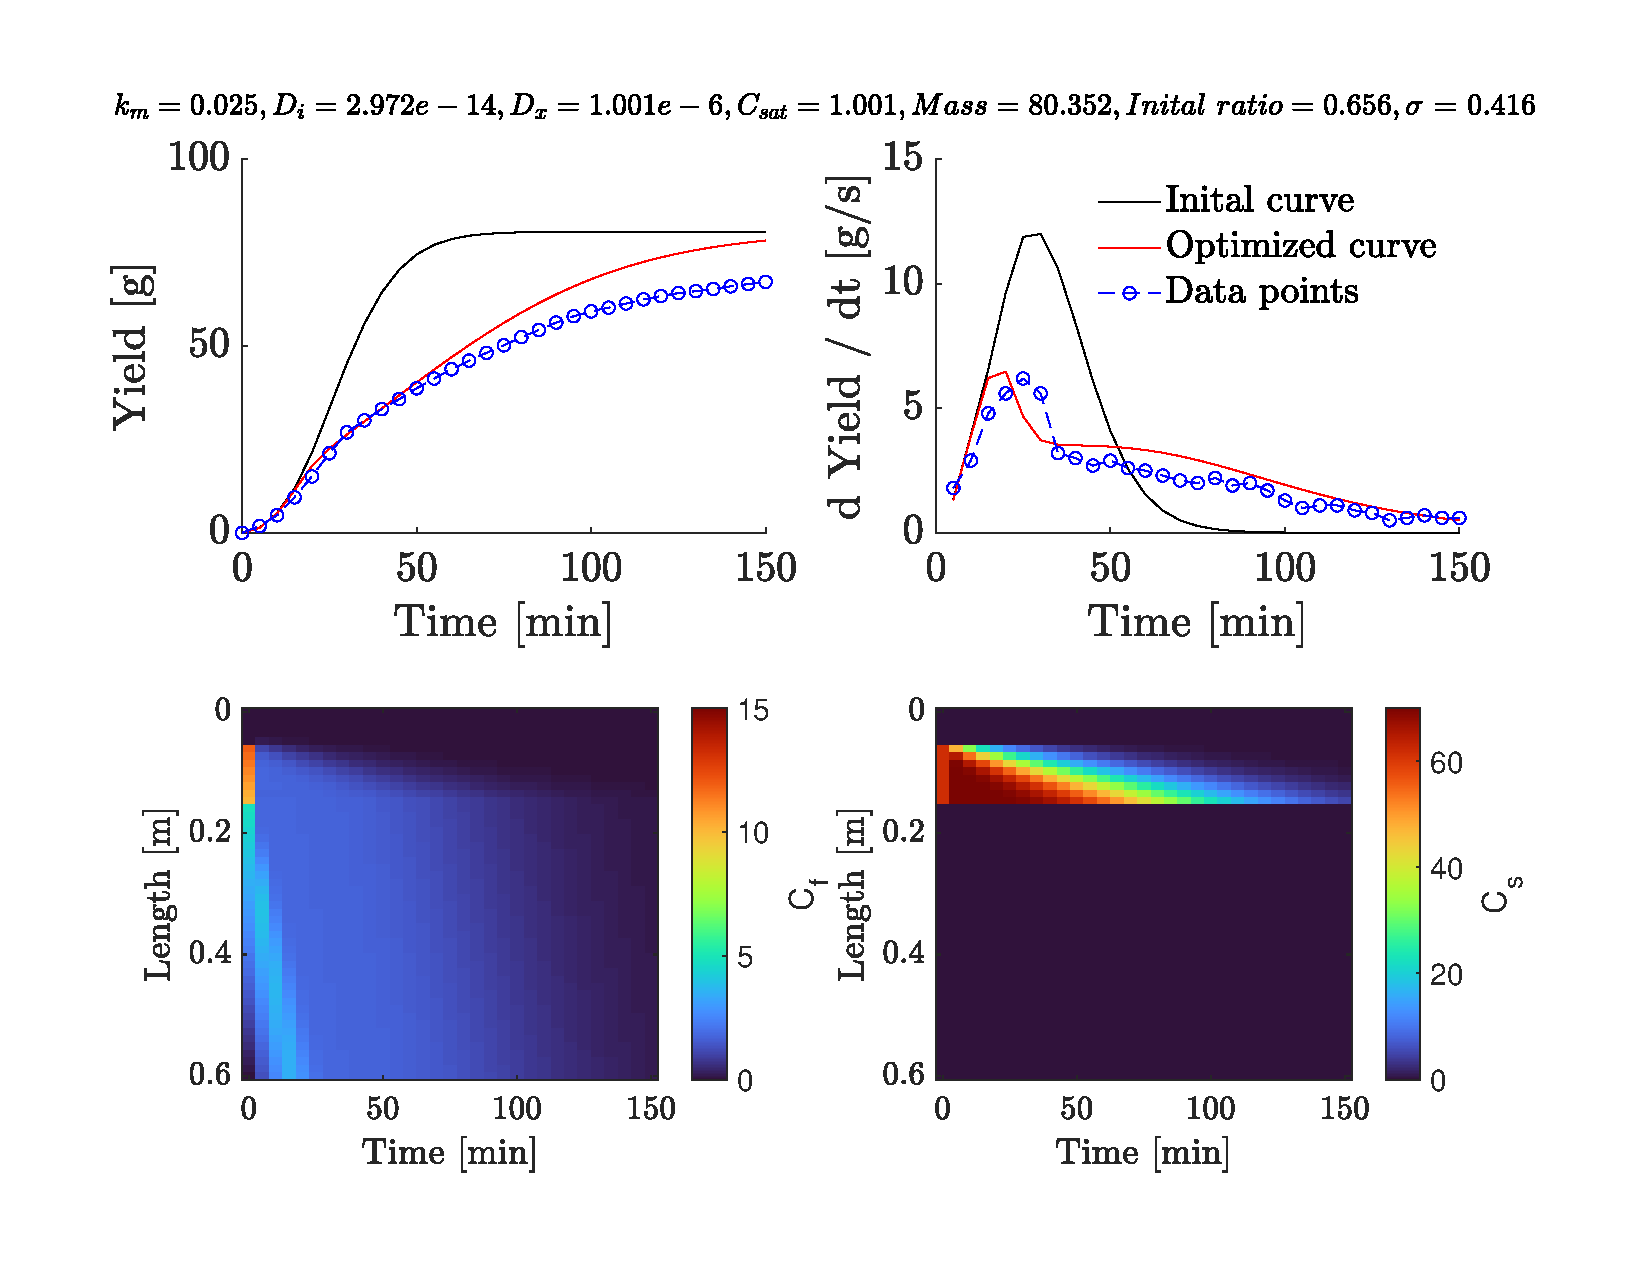
\includegraphics[trim = 3cm 11cm 2.5cm 1cm,clip,width=\textwidth]{/Results_estimation/Fitting_LUKE_T50_P200.pdf}
			\caption{Experiment at $50^\circ C$ and $200$ bar}
		\end{subfigure}
		\hfill
		\begin{subfigure}[b]{0.7\textwidth}
			\centering
			\includegraphics[trim = 3cm 11cm 2.5cm 1cm,clip,width=\textwidth]{/Results_estimation/Fitting_LUKE_T40_P300_org.pdf}
			\caption{Experiment at $40^\circ C$ and $300$ bar}
		\end{subfigure}
		\hfill
		\begin{subfigure}[b]{0.7\textwidth}
			\centering
			\includegraphics[trim = 3cm 11cm 2.5cm 1cm,clip,width=\textwidth]{/Results_estimation/Fitting_LUKE_T50_P300_org.pdf}
			\caption{Experiment at $50^\circ C$ and $300$ bar}
		\end{subfigure}
		\caption{Results of parameter fitting, with estimation of the initial state}
	\end{figure*}

	\begin{figure*}
	\centering
	\begin{subfigure}[b]{0.85\textwidth}
		\centering
		\includegraphics[trim = 1cm 2cm 2.5cm 1cm,clip,width=\textwidth]{/Results_estimation/Trend_Lines_order_1.pdf}
		\caption{First order polynomial regression of fitted parameters as a function of fluid density $\rho_f$}
	\end{subfigure}
	\hfill
	\begin{subfigure}[b]{0.85\textwidth}
		\centering
		\includegraphics[trim = 1cm 2cm 2.5cm 1cm,clip,width=\textwidth]{/Results_estimation/Trend_Lines_order_2.pdf}
		\caption{Second order polynomial regression of fitted parameters as a function of fluid density $\rho_f$}
	\end{subfigure}
	\caption{Results of parameter fitting, with estimation of the initial state}
\end{figure*}
		
	
\end{document}